\section{Теоритические сведения}
\subsection{Дифракция}
Дифракцией называются отклонения в распространении волн от законов геометрической оптики.

Основными параметрами, определяющими характер дифракционных явлений, является длина волны $\lambda$, размер отверстия $b$ и расстояние до плоскости наблюдения $z$. Характер дифоракции определяется волновым параметром

\[
    p = \frac{\sqrt{\lambda z}}{b}
\]

При $p \ll 1$ выполняются законы геометрической оптики, при $p\approx 1$ происзодит дифракция Френеля, $p\gg 1$~--- дифракция Фраунгофера.

\subsection{Принцип Гюйгенса-Френеля}
\begin{figure}[ht!]
    \center{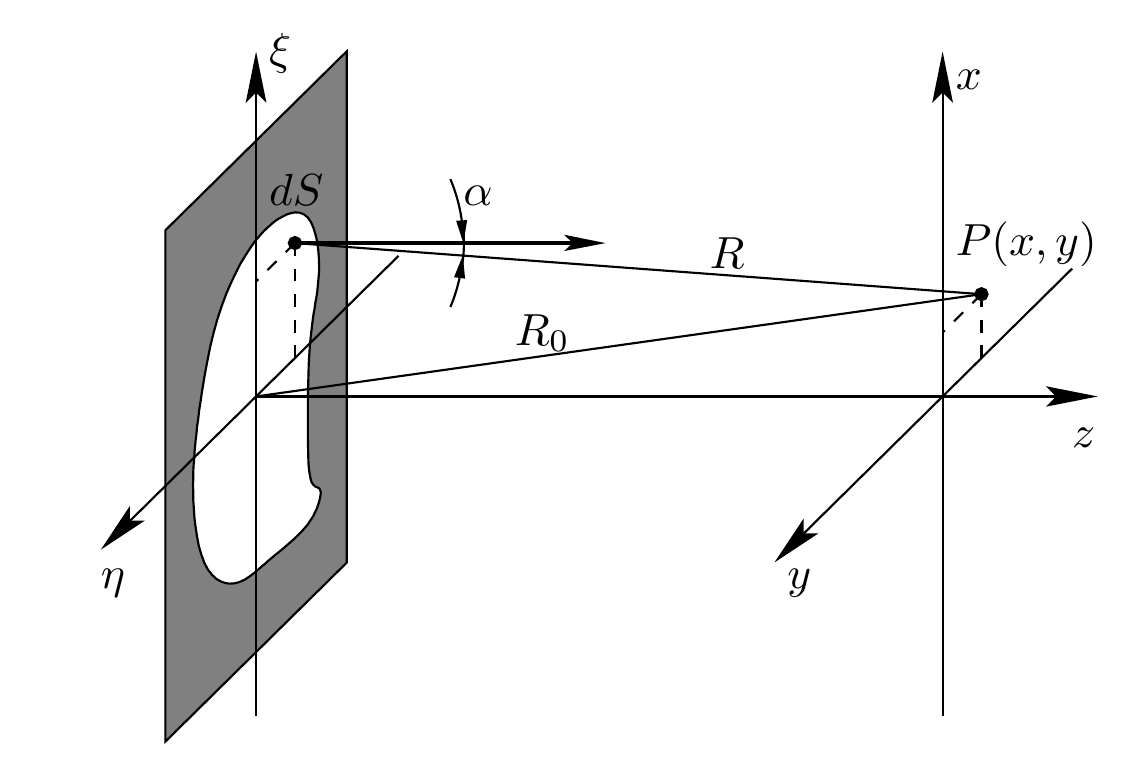
\includegraphics[width=0.8\linewidth]{../img/gufr.png}}
\end{figure}

Пусть волна света, созданная источниками, расположенными в области $z < 0$, достигла плоскости $z=0$. Световое поле в этой плоскости нам известно. Пусть его комплексная амплитуда есть
\[
    f_{0}(x, y) = a_{0}(x, y)e^{i \varphi_{0}(x, y)}
\]
где функции $a_{0}(x, y)$ и $ \varphi_{0}(x, y)$ описывают распределение амплитуд и фаз колебаний в плоскости $z=0$.

Согласно принципу Гюйгенса, каждую точку $( \xi, \eta)$ плоскости $z = 0$, куда пришла волна, можно рассматривать  как источник вторичной волны. То есть можно представить себе, что волна возбуждает колебания некоторого фиктивного источника (осциллятора), который и переизлучает вторичную волну. Частота $ \omega$ этой переизлучённой волны совпадает с частотой исходной монохроматической волны. Френель дополнил принцип Гюйгенса, предложив рассматривать световое колебание в любой точке наблюдения в области $z > 0$ как результат интерференции этих вторичных волн.

Предполагается, что амплитуда излучения вторичного источника пропорциональна амплитуде $a_{0}(\xi, \eta)$  колебания, созданного реальной волной, пришедшей к площадке $ds$. Фаза колебания также задаётся фазой $ \varphi( \xi, \eta)$ пришедшей к элементу $ds$ волны.

Далее предполагается, что маленькая площадка $ds$ переизлучает, подобно точечному источнику, сферическую волну, т. е. для вычисления вклада, который даёт эта площадка в суммарное колебание в точке наблюдения $P$,  нужно учесть ослабление амплитуды и набег фазы $e^{ikR}/R$. Наконец, предполагается, что амплитуда колебания пропорциональна видимой из точки наблюдения площади элемента $ds$, т.е. пропорциональна $ds\cos\alpha$. Таким образом, вклад элемента $ds$ пропорционален величине
\[
    f_{0}(\xi, \eta)\frac{e^{ikR}}{R}\cos\alpha\cdot d\xi d\eta
\]
Полное световое колебание $g(x, y)$ есть результат интерференции всех вторичных волн, посылаемых всеми площадками $ds$, расположенными в области отверстия:
\[
    g(x, y) = \frac{1}{i\lambda}\iint_{S} f_{0}(\xi, \eta)\frac{e^{ikR}}{R}\cos\alpha d\xi d\eta
\]

При условии, что размер препятствия мал по сравнению с расстоянием $R_{0}$ до точки наблюдения, амплитудный множитель $\frac{1}{R}$,  учитывающий уменьшение амплитуды в сферической волне по мере удаления от вторичного источника $ds$, можно заменить постоянной величиной $\frac{1}{R_{0}}$. Множитель наклона $\cos\alpha$ также считаем приблизительно одинаковым (и равным единице) для всех вторичных источников, расположенных в области отверстия. Тогда в этом приближении принцип Гюйгенса—Френеля приобретает следующий вид:
\[
    g(x, y) = \frac{1}{i\lambda R_{0}} \iint f_{0}(\xi, \eta)e^{ikR} d\xi d\eta
\]
\[
    R \approx z + \frac{\left(x - \xi\right)^{2}}{2z} + \frac{\left(y - \eta\right)^{2}}{2z}
\]

Тогда
\[
    g(x, y) = \frac{e^{ikz}}{i \lambda z}\iint f_{0}(\xi, \eta)e^{i\frac{k}{2z}\left(\left(x-\xi\right)^{2} + \left(y - \eta\right)^{2}\right)} d\xi d\eta
\]
Если отверстиеосвещается плоской волной, то $f_{0}(\xi, \eta) = A_{0}$.

\section{Теоритические сведения}
\subsection{Спектральный метод решения задачи дифракции}
Спектральные методы являются основой при изучении колебаний различной физической природы (электрический колебательный контур, механический осциллятор, электрон в атоме и т.д.). Суть спектрального метода состоит в представлении внешнего воздействия, возбуждающего колебания в линейной системе, в виде суммы некоторых элементарных воздействий. Свойство линейности системы (принцип
суперпозиции) позволяет найти решение задачи в виде соответствующей суммы откликов --- вынужденных колебаний, возбуждаемых в
системе отдельным элементарным воздействием. Важнейшей проблемой при использовании спектрального метода является проблема поиска <<<базиса>>> --- элементарных слагаемых. При изучении стационарных
колебательных линейных систем широко используется представление внешнего воздействия $f(t)$ в виде суммы гармонических колебаний различных частот $\omega_n$: $f(t) = \sum c_n e^{i\omega_n t}$. Особая роль гармонических слагаемых $e^{i\omega t}$ обусловлена тем, что гармоническое внешнее воздействие $e^{i\omega t}$ возбуждает в линейной стационарной системе процесс вынужденных колебаний, которые также являются гармоническими и частота которых совпадает с частотой внешнего воздействия.

Применим спектральный метод к исследованию законов распространения волн в задаче дифракции (метод Рэлея), основанный на представлении пространственной структуры дифрагированной волны в виде суперпозиции плоских волн разных направлений.

\subsection{Распространение плоской волны}
Рассмотрим плоскую волну, волновой вектор которой $\vec{k}$ составляет угол $\alpha$ с осью $z$. Комплексная амплитуда такой волны имеет вид
\[
f(x,z) = ae^{i(k_xx+k_zz+\varphi)}
\]
$a$ --- амплитуда, $\varphi$ --- начальная фаза, $k_x$ и $k_z$ --- проекции $\vec{k}$ на оси $x$ и $z$ ($k_y = 0$).

\begin{figure}[ht!]
    \center{
\includegraphics[width=0.8\linewidth]{../img/vawe1.png}}
\end{figure}

Введём комплексный коэффициент $c = ae^{i\varphi}$ и обозначение $k_x = u$. Тогда, имея в виду, что $k_x^2 + k_z^2 = k^2$
\[
f(x, z) = ce^{i(ux + \sqrt{k^2 - u^2}\cdot z)}
\]
Волновое поле плоской волны в любой плоскости $z > 0$ можно найти, если известно поле плоской волны в плоскости $z=0$:
\[
    f(x, 0) = ce^{iux}
\]
откуда
\[
    f(x, z) = f(x, 0)\cdot e^{i\sqrt{k^2-u^2}z},
\]
т.е. комплексные амплитуды $f(x, 0)$ и $f(x, z)$  отличаются множителем $H(u) = e^{i\sqrt{k^2 - u^2}\cdot z}$,  определяющим набег фазы плоской волны прираспространении между двумя плоскостями, разделенными промежутком $z$.

Обратим внимание на аналогию с выражением $f(t) = ce^{i\omega t}$, которое, как мы знаем, есть не что иное, как комплексная форма записи гармонического колебания частоты $\omega$, причём комплексный множитель $c$ определяет амплитуду колебания и его начальную фазу. На основании этой аналогии величина $u=k\sin\alpha$  может быть названа пространственной частотой. Можно сказать, что волны разных направлений $\alpha$ --- это волны разных пространственных частот.

\subsection{Спектр плоских волн}
Итак, представим граничное поле $f_0(x)$ в виде суммы плоских волн:
\[
f_0(x) = \sum c_n e^{iu_nx}
\]

Набор чисел $c_n$ представляет собой пространственный спектр волнового поля $f_0$.  Каждое слагаемое в сумме есть поле плоской волны при $z=0$, направление $\alpha_n$ которой определяется пространственной частотой $u_n = k\sin\alpha_n$.  Подчеркнём, что частота волн $\omega$ предполагается заданной и, следовательно, волновое число$k = \omega / v$ всех плоских волн в пространственном разложении одинаково.

Напомним, что в общем случае произвольное граничное поле $f_0(x)$ представляется в виде интеграла Фурье:
\[
f_0(x) = \frac{1}{2\pi}\int C_0 (u) e^{iux} du,
\]
т.е. в виде непрерывной суммы плоских волн различных пространственных частот. Функция $C_0(u)$ есть преобразование Фурье функции $f_0(x)$. Пространственный спектр $C_0(u)$ (его можно назвать спектром плоских волн) определяется соотношением
\[
    C_0(u) = \int_{-\infty}^{+\infty} f_0(x)e^{-iux}dx
\]

Напомним также, что если функция $f_0(x)$ периодична по координате $x$, то она представляется рядом Фурье:
\[
    f_0(x) = \sum_n c_n e^{inu_0x}
\]
\[
    c_n = \frac{u_0}{2\pi}\int_{-d/2}^{d/2} f_0(x)e^{-inu_0x}dx
\]

\subsection{Распространение волн}
Важно подчеркнуть, что речь идёт о линейной задаче: распространение волны от плоскости $z=0_+$  до плоскости наблюдения $z > 0$ описывается линейным волновым уравнением  или, поскольку мы пользуемся комплексным представлением, линейным уравнением Гельмгольца. Основное свойство линейного уравнения: сумма решений является решением.

Вспомним теперь, что плоская волна
\[
    f_n(x, z) = c_n e^{i(u_nx + \sqrt{k^2-u_n^2}z)}
\]
есть решение уравнения Гельмгольца, удовлетворяющее на плоскости $z=0_+$ граничному условию
\[
    f_n(x, 0) = c_n e^{iu_nx}
\]
поэтому сумма плоских волн
\[
    f(x,z) = \sum_n c_n e^{i(u_nx + \sqrt{k^2-u_n^2}z)}
\]
есть решение, удовлетворяющее граничному условию.

В общем случае, если граничное поле $f_0(x)$ представляется непрерывной суперпозицией плоских волн, искомое решение имеет вид
\[
    f(x,z) = \int C_0(u) e^{i(ux+\sqrt{k^2-u^2}z)} du
\]
$C_0(u)$~--- преобразование Фурье граничного поля $f_0(x)$.

Существенным является следующее обстоятельство: каждая слагаемая плоская волна при распространении до плоскости наблюдения $z > 0$ приобретает свой фазовый набег $\varphi_n = \sqrt{k^2 - u_n^2}\cdot z$, зависящий от ее пространственной частоты $u_n$. Поэтому фазовые соотношения между слагаемыми плоскими волнами на границе $z=0$ и в плоскости наблюдения, отстоящей на расстоянии $z$,  различны. Изменение фазовых соотношений между слагаемыми плоскими волнами приводит к тому, что изменяется результат интерференции этих волн. Поэтому результирующее поле $f(x,z)$ в плоскости наблюдения может кардинально отличаться от граничного поля $f_0(x)$ (хотя и то, и другое составлено из суперпозиции тех же бегущих плоских волн).

\subsection{Передаточная функция}
\[
f(x,z) = \int C_0(u) e^{i\sqrt{k^2-u^2}z}e^{iux}du = \int C(u,z)e^{iux}du
\]
Функция
\[
C(u,z) = C_0(u) e^{i\sqrt{k^2-u^2}z}
\]
представляет собой преобразование Фурье (пространственный спектр) монохроматического волнового поля $f(x,z)$ в плоскости наблюдения.

Множитель
\[
H(u) = e^{i\sqrt{k^2-u^2}z}
\]
связывающий пространственные спектры $C_0(u)$ и $C(u, z)$ волнового поля в двух плоскостях, разделённых промежутком свободного пространства $z$, называют передаточной функцией (или частотной характеристикой) свободного пространства (точно так же частотная характеристика $H(\omega)$  связывает между собой спектры входного и выходного сигнала линейного временного фильтра). Поэтому участок свободного пространства можно рассматривать как простейший линейный пространственный фильтр, входным сигналом которого является поле $f_0(x)$ во входной плоскости $z=0_+$, а выходным сигналом --- поле $f(x,z)$ в выходной плоскости $z>0$.

Во многих задачах речь идёт о волновых полях, имеющих достаточно узкий спектр плоских волн $|U| \ll k$. При этом используют приближённое выражение для частотной характеристики:
\[
H(u) \approx e^{ikz}e^{-izu^2/2k}
\]
которое получается разложением радикала $\sqrt{k^2-u^2}$ в ряд по степеням малого параметра $(u / k)^2$, причём удерживаются лишь два члена разложения:
\[
\sqrt{k^2-u^2} \approx kz - \frac{z}{2k}u^2
\]
При этом точное равенство заменяется приближённым:
\[
C(u, z) \approx C_0(u)e^{-izu^2/2k}
\]

Итак, метод Рэлея предлагает следующую последовательность решения задач дифракции.

Зная поле сторонних источников $f_s(x)$ и функцию пропускания транспаранта $t(x)$, находим с помощью граничных условий граничное поле $f_0(x)$.

Определяем пространственный  спектр граничного поля: набор коэффициентов $c_n$ ряда Фурье либо фурье-образ $C_0(u)$ функции $f_0(x)$.

 Наконец, определяем искомое поле $f(x, z)$ на расстоянии $z$ от препятствия ---  тонкого экрана.

\subsection{Дифракция Френеля на амплитудной синусоидальной решётке}
Функция пропускания решётки с периодом $d=pi/\Omega$:
\[t(x) = 1 + m\cos\Omega x\]
Пусть решётка освещается плоской нормально падающей волной амплитуды $a$: $f_s(x) = ae^{ikz}$. Решётка установлена в плоскости $z=0$, поэтому $f_s = a$. Тогда, согласно граничным условиям
\[
f_0(x) = a(1 + m\cos\Omega x) = a + \frac{am}{2} e^{i\Omega x} + \frac{am}{2} e^{-i\Omega x}
\]

Комплексная амплитуда волны в плоскости $z$ имеет вид
\[
f(x, z) = ae^{ikz} + \frac{am}{2}e^{i(\Omega x + \frac{k^2-\Omega^2}z)} + \frac{am}{2}e^{i(-\Omega x + \frac{k^2-\Omega^2}z)}
\]
каждое слагаемое в граничном поле ответственно за свою волну в области $z>0$.  Первое слагаемое --- волна с амплитудой $a$, бегущая вдоль оси $z$. Два других слагаемых --- волны с амплитудами $am/2$ и пространственными частотами $\pm \Omega$. Эти волны бегут в направлениях $\sin\alpha = \pm \Omega / k = \pm \lambda / d$. Отметим, что в начале координат $x=0$ в плоскости $z=0_+$ все три волны создают синфазные колебания.

Полагаем, что период решётки $d = \frac{2\pi}{\Omega}$ существенно больше длины волны $\lambda$ и, следовательно, $\Omega \ll k$.

\[
f(x,z) = ae^{ikz} + \frac{am}{2}e^{ikz} \cdot e^{i(\Omega x - \frac{z}{2k}\Omega^2)} + \frac{am}{2}e^{ikz} \cdot e^{i(-\Omega x - \frac{z}{2k}\Omega^2)} = ae^{ikz}\left(1 + me^{-i\frac{z}{2k}\Omega^2}\right)\cdot \cos \Omega x
\]
Последнюю формулу можно использовать для анализа картины дифракции на различных расстояниях $z$ от решётки.

На расстояниях $z_n = \frac{2d^2}{\lambda}n$ имеем $e^{-i\frac{z_n}{2k}\Omega^2} = 1$, поэтому $f(x, z) = e^{ikz_n}f_0(x)$, т.е. с точностью до фазового множителя воспроизводится граничное поле $f_0(x)$. Воспроизводится, разумеется, наблюдаемая картина интенсивности $I(x, z_n) = I_0(x)$.
\[
I(x, z_n) = |f(x, z_n)|^2 \approx a^2(1 + 2m\cos\Omega x)
\]
\[
V = \frac{I_{max} - I_{min}}{I_{max} + I_{min}} \approx 2m
\]

На расстояниях $z_n = \frac{d^2}{\lambda}(2n + \frac{1}{2})$ $f(x, z) = a(1 + im\cos\Omega x)$. $I \approx a^2$, $V \approx 0$.

Таким образом, периодически по $z$ изменяется видность наблюдаемой дифракционной картины. Причина этих изменений --- в различии фазовых набегов трёх плоских волн, бегущих в области $z > 0$ от решётки: осевой волны, бегущей вдоль оси $z$, и двух боковых волн, бегущих в направлениях $\sin\alpha = \pm \Omega / k = \pm \lambda / d$.

\subsection{Дифракция Френеля на периодических структурах}
Примером периодической структуры является экран с периодически расположенными одинаковыми элементами, например, параллельными щелями одинаковой ширины  $b$, расположенными на одинаковом расстоянии $d$ друг от друга. Пусть такой экран (решётка) освещается слева плоской нормально падающей волной.

На выходе из экрана(в плоскости, примыкающей к нему справа) получаем световое поле, комплексная амплитуда которого $f_0(x)$ является периодической функцией с периодом $d$, которую можно представить в виде ряда Фурье:
\[
f_0(x) = \sum c_n e^{in\frac{2\pi}{d}x}
\]
Каждое слагаемое ряда представляет собой поле плоской волны, пространственная частота которой $u_n = n\frac{2\pi}{d}$ определяет направление волнового вектора $\vec{k}_n$ ($u_n = k\sin\alpha_n$) этой волны, т.е. $\sin\alpha_n = n\frac{\lambda}{d}$. Комплексная амплитуда волны в плоскости наблюдения, отстоящей на расстоянии $z$  от решётки, имеет вид
\[
f(x, z) = \sum c_ne^{i(u_nx + \sqrt{k ^ 2 - u_n^2}z)}
\]
Фаза $n$-й  плоской волны в плоскости $z$  равна $\varphi_n = \sqrt{k^2 - u_n^2}z \approx kz - \frac{zu_n^2}{2k}$. Сравним набег фазы $n$-й плоской волны с набегом фазы $\varphi_0$ плоской волны, бегущей вдоль оси $z$: $\varphi_0 = kz$. Мы получаем
\[
\Delta\varphi_n = \varphi_0 - \varphi_n = \frac{z}{2k}\left(\frac{2\pi n}{d}\right)^2 = \pi \frac{\lambda z}{d^2} n^2
\]
Рассмотрим плоскость наблюдения, отстоящую от плоскости решётки на расстояние
\[
    z_1 = \frac{2d^2}{\lambda}
\]
В этом случае $p \approx 1$ и имеет место дифракция Френеля. В этой плоскости имеем $\Delta \varphi_n = 2\pi n^2$. Очевидно, что и разность фазовых набегов любых двух волн, равная $2\pi(n_1^2 - n_2^2)$, также кратна $2\pi$. Но изменение разности фаз колебаний на величину, кратную $2\pi$, ничего не меняет в суммарном колебании. Мы пришли к замечательному результату: фазовые соотношения между слагаемыми плоскими волнами оказались одинаковыми как в плоскости, примыкающей к решётке, так и в плоскости $z$. Одинаковость фазовых соотношений слагаемых плоских волн приводит к тому, что одинаков и результат интерференции этих плоских волн, т.е. световое поле в плоскости $z_1$ отличается от граничного поля $f_0$ лишь постоянным фазовым множителем $e^{ikz}$.

Мы наблюдаем в плоскости $z_1$  периодическую структуру, тождественно повторяющую граничное поле $f_0$. Очевидно также, что такое восстановление изображения периодической структуры повторяется на расстояниях, кратных $z_1$:
\[
z_m = m\frac{2d^2}{\lambda}
\]
Описанный эффект называют эффектом самовоспроизведения, или эффектом Талбота.

\subsection{Спектр плоских волн при дифракции на щели}

\begin{figure}[ht!]
    \center{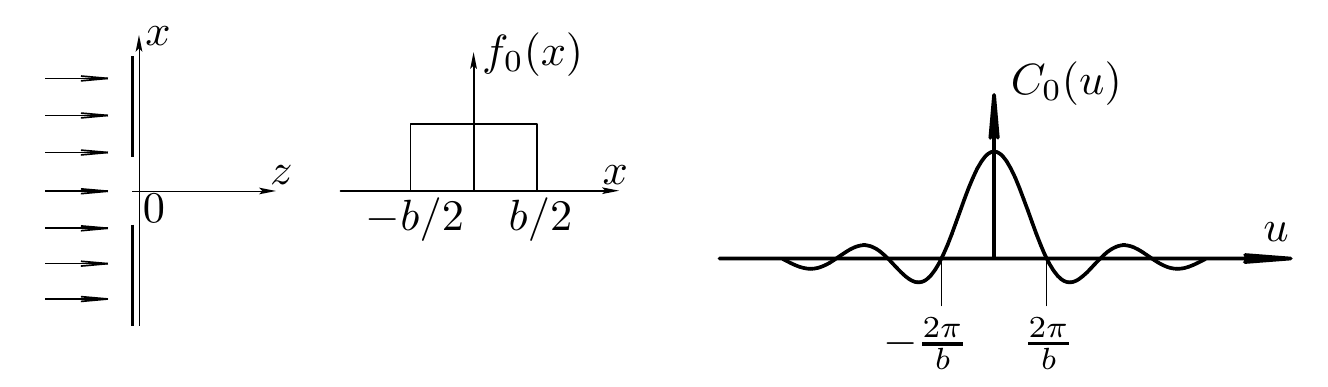
\includegraphics[width=0.8\linewidth]{../img/wave2.png}}
\end{figure}

Пусть щель в непрозрачном экране (ширина щели $b$) освещается нормально падающей плоской волной единичной амплитуды. Тогда в плоскости $z=0_+$, примыкающей к щели справа от неё, имеем
\[
f_0(x) = I_{|x| \le b}
\]
Пространственный спектр граничного поля
\[
C_0(u) = b\frac{\sin bu / 2}{bu / 2}
\]
Спектр $C_0(u)$ показан на рисунке. Область значений $\Delta u$, в которой функция заметно отлична от нуля, называют обычно шириной спектра.
\[
|\Delta u| \approx \frac{2\pi}{b}
\]
В общем случае справедливо соотношение неопределённостей
\[
\Delta x \cdot \Delta u \approx 2\pi
\]
Пространственная протяжённость граничного поля определяется характерным размером препятствия, в нашем примере --- размером $b$ отверстия в непрозрачном экране. Разброс пространственных частот определяет разброс направлений слагаемых плоских волн за отверстием:
\[
\Delta u = k \Delta \sin\alpha
\]
Отсюда получаем дифракционную расходимость пучка
\[
\Delta\alpha \approx \frac{\lambda}{b}
\]

\subsection{Поле в фокальной плоскости линзы. Пространственное преобразование Фурье}
Как известно, линза фокусирует параллельный пучок света: плоская волна, бегущая в направлении $\alpha$, т.е. имеющая пространственную частоту $u = k\sin\alpha$, фокусируется линзой в точку фокальной плоскости с координатой
\[
x = f\tg \alpha \approx f\sin\alpha = \frac{fu}{k}
\]
Имеется, как мы видим, взаимно однозначное соответствие между точками фокальной плоскости и пространственными частотами плоских волн, которые в эти точки фокусируются. Оказывается, взаимно однозначное соответствие имеет место также и между амплитудами и фазами колебаний в точках фокальной плоскости и соответствующих им плоских волн.

\begin{figure}[ht!]
    \center{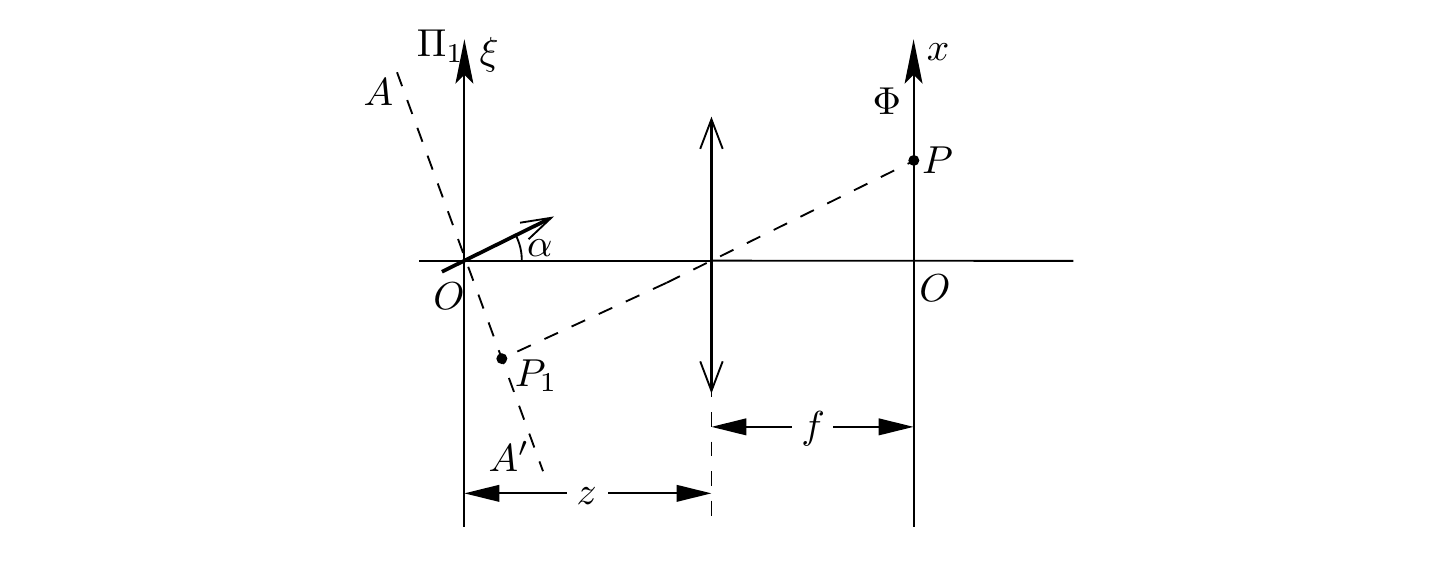
\includegraphics[width=0.8\linewidth]{../img/furry1.png}}
\end{figure}

Пусть на линзу падает произвольная волна. Во входной плоскости $\Pi_1$, отстоящей от линзы на расстоянии $z$,  волна имеет комплексную амплитуду $f_0(x)$. Представим эту волну в виде суперпозиции плоских волн разных направлений $\alpha_n$. Плоская волна $c_n e^{iu_nx}$, соответствующая одному из слагаемых, показана на рисунке: её волновой вектор составляет угол $\alpha = \alpha_n$ ($\sin\alpha = \frac{u_n}{k}$) с оптической осью. Коэффициент $c_n = a_n e^{i\varphi_n}$ определяет амплитуду плоской волны $a_n$ и начальную фазу $\varphi_n$.

Очевидно, что амплитуда колебаний в точке $P$ фокальной плоскости пропорциональна амплитуде $a_n$ плоской волны, которая в эту точку сфокусировалась. Найдём, каковы фазовые соотношения между колебаниями в разных точках фокальной плоскости. Ясно, что колебание в точке $P$  отстаёт по фазе от колебания в точке $P_1$, причём разность фаз определяется длиной оптического пути $P_1P$: прямая $P_1P$ перпендикулярна в каждой точке волновым поверхностям ---  плоским поверхностям в волне, падающей на линзу, и сферическим в волне, прошедшей через линзу.  Пусть соответствующая пути $P_1P$ задержка по фазе равна $\psi_n$. Тогда фаза колебания в точке $P$ фокальной плоскости равна $\varphi_n + \psi_n$, а комплексную амплитуду колебаний в этой точке можно записать в виде $f(x_n) = c_ne^{i\psi_n}$.

Слагаемому $c_0e^{iu_0x}$ соответствует плоская волна, бегущая вдоль оптической оси. Она фокусируется в начало координат $x=0$ фокальной плоскости Ф. Коэффициент $c_0 = a_0e^{i\varphi_0}$ определяет амплитуду $a_0$ этой волны и её начальную фазу $\varphi_0$, т.е. фазу колеюаний в точке O входной плоскости $\Pi_1$. Задержка по фазе $\psi_0$ в точке $x=0$ фокальной плоскости Ф, куда эта волна сфокусировалась, определяется длиной оптического пути $OO$. Комплексная амплитуда колебаний в этой точке есть $f(0) \approx c_0 e^{i\psi_0}$.

Пусть $z = f$, т.е. плоскость $\Pi_1$ --- это передняя фокальная плоскость линзы. Легко видеть, что в приближении малых углов оптические пути $P_1P = z\cos\alpha + \frac{f}{\cos\alpha} + \Delta_0$ и $OO = z + f + \Delta_0$ ($\Delta_0$~--- оптический путь, проходящий непосредственно через линзу на главной оптической оси) равны при $z=f$, т.е. $\psi_n = \psi_0$.

Одинаковость для всех плоских волн фазовых задержек $\psi_n$ означает, что фазовые соотношения между колебаниями в разных точках задней фокальной плоскости, куда эти волны сфокусировались, таковы же, как и фазовые соотношения между колебаниями, которые создают эти волны в начале координат передней фокальной плоскости. Таким образом, волновое поле в задней фокальной плоскости линзы правильно воспроизводит не только амплитудные соотношения между плоскими волнами разных пространственных частот, но и фазовые соотношения без искажений, т.е. картина поля в фокальной плоскости воспроизводит пространственный спектр (пространственное преобразование Фурье) падающей на линзу волны.

Опуская несущественный постоянный фазовый множитель $e^{i\psi_0}$, получаем $f(x_n) = c_n = C(\frac{kx_n}{f})$. Последнее равенство справедливо для любой точки $x_n$  фокальной плоскости. Если спектр плоских волн непрерывен, т. е. волна, падающая на линзу, состоит из плоских волн любых направлений, то, опуская индекс $n$, находим
\[
f(x) = C\left(\frac{kx}{f}\right) = \int f_0(\xi) e^{-i\frac{kx}{f}\xi} d\xi
\]
где $C(u)$~--- преобразование Фурье поля $f_0(x)$. Итак, световое поле в задней фокальной плоскости линзы $f(x)$ связано с полем волны, падающей на линзу $f_0(\xi)$, преобразованием Фурье.

Если комплексная амплитуда волны, падающей на линзу, задаётся в произвольной плоскости на расстоянии $z \ne f$ от линзы, то легко получить
\[
    f(x) = exp\left(i\frac{k}{2f}(1 - z / f)x^2\right) \cdot C\left(\frac{kx}{f}\right)
\]

т.е. возникают фазовые искажения, обусловленные дополнительным набегом фазы $\varphi(u) = \sqrt{k^2 - u^2}\Delta z$, который приобретает плоская волна, пробегая промежуток свободного пространства, равный $\Delta z = z - f$. Важно обратить внимание, что наблюдаемая картина интенсивности
\[
I(x) = \left|C\left(\frac{kx}{f }\right)\right|^2
\]
не зависит от $z$.

\subsection{Принцип двойной дифракции и формирование оптического изображения (теория Аббе)}

\begin{figure}[ht!]
    \center{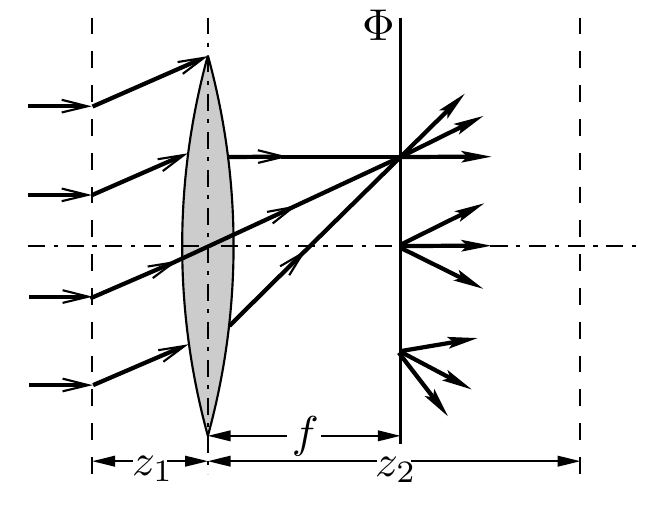
\includegraphics[width=0.4\linewidth]{../img/ab1.png}}
\end{figure}

Формирование изображения с помощью линзы можно рассматривать, основываясь на идее пространственного спектрального разложения. Монохроматическую волну, идущую от предмета, представим в виде суперпозиции плоских волн разных направлений $\alpha$, т.е.  разных пространственных частот $u=k\sin\alpha$. Каждая гармоника --- плоская волна определённого направления --- фокусируется линзой в свою точку фокальной плоскости, в которой возникает, таким образом, картина пространственного спектра: амплитуда и фаза колебаний в точке $\xi$ фокальной плоскости однозначно определяются амплитудой и фазой колебаний той плоской волны, которая в эту точку фокусируется.

По этой причине фокальную плоскость линзы называют фурье-плоскостью. По терминологии Аббе, впервые предложившего такой подход, поле в фокальной плоскости называют первичным изображением. На рисунке показана ситуация, когда предметом является решётка, освещаемая плоской нормально падающей волной. При этом в фурье плоскости, как мы знаем, возникает картина фраунгоферовой дифракции: набор ярких точек --- дифракционных максимумов. Итак, в процессе распространения света от предмета до фурье плоскости осуществляется преобразование Фурье светового поля.

Далее каждая точка фурье-плоскости рассматривается как источник сферической волны. Все сферические волны, исходящие из разных точек фурье-плоскости, интерферируя, образуют в плоскости, находящейся на расстоянии $z_2$ за линзой, собственно изображение объекта. Это изображение Аббе назвал вторичным, а процесс распространения света от фурье-плоскости до плоскости изображения --- второй дифракцией.

\begin{figure}[ht!]
    \center{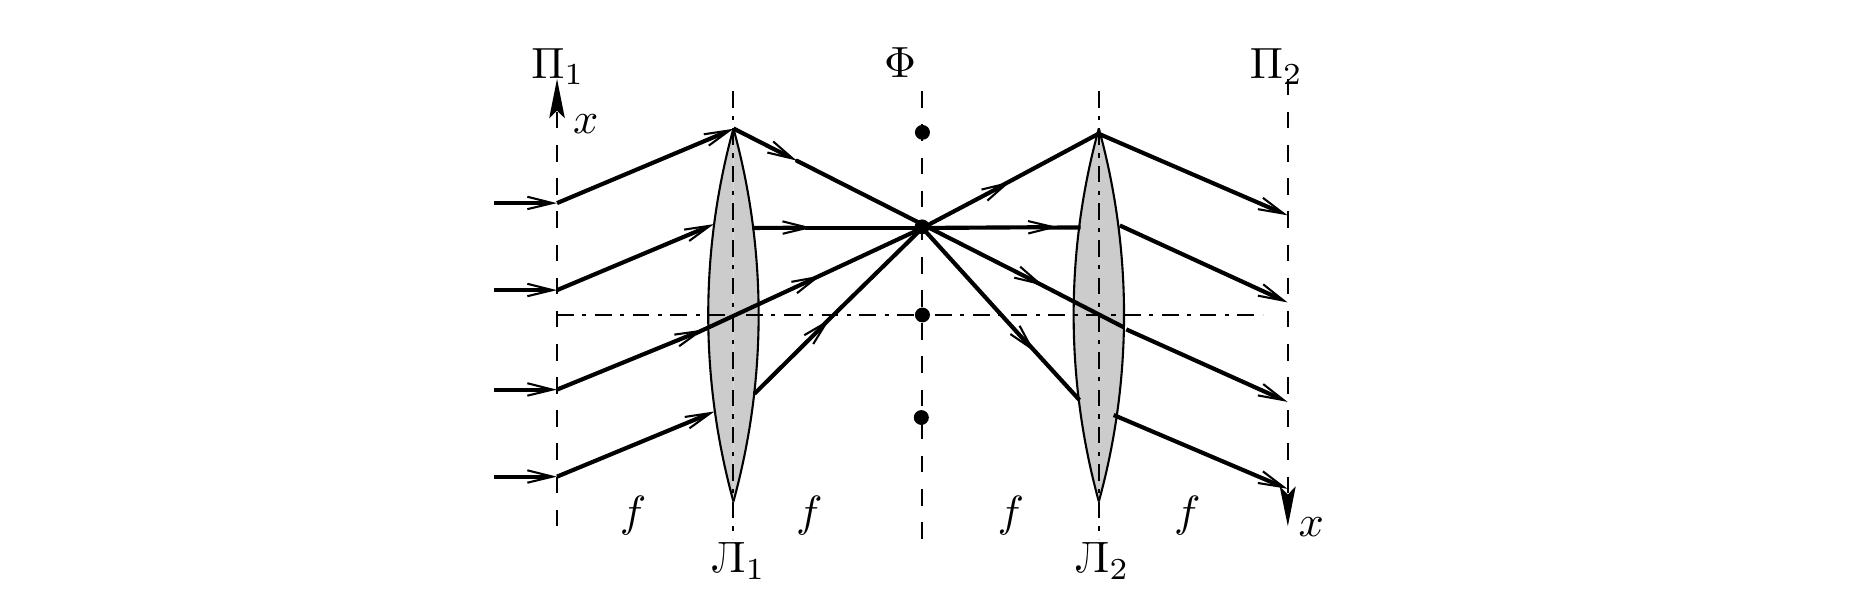
\includegraphics[width=0.8\linewidth]{../img/ab2.png}}
\end{figure}

Особенно наглядно принцип двойной дифракции проявляется в оптической схеме, показанной на рисунке. Схема состоит из двух линз с общей фокальной плоскостью Ф. Задняя фокальная плоскость линзы $\text{Л}_1$ совпадает с передней фокальной плоскостью линзы $\text{Л}_2$. В этом случае первая дифракция --- это распространение света от передней фокальной плоскости линзы $\text{Л}_1$, где расположен предмет, к плоскости Ф, где возникает картина пространственного спектра --- первичное изображение. Далее, сферическая волна, идущая из любой точки фурье-плоскости, преобразуется линзой $\text{Л}_2$ в плоскую волну. Таким образом, каждая плоская волна, идущая от предмета, преобразуется системойдвух линз в плоскую волну, приходящую к плоскости изображения. Причем, если фокусные расстояния линз одинаковы, то волна с пространственной частотой $u = k\sin\alpha$ преобразуется в волну с пространственной частой $-u$. Это приводит к инверсии --- изображение оказывается перевёрнутым. Можно сказать, что в процессе образования изображения происходит два последовательных преобразования Фурье: от входной плоскости $\Pi_1$ к фурье-плоскости --- первая дифракция, и затем от фурье-плоскости с помощью линзы $\text{Л}_2$ к выходной плоскости $\Pi_2$ --- вторая дифракция.

\subsection{Пространственная фильтрация}
Особая роль фурье-плоскости обусловлена тем, что именно в этой плоскости возможно избирательное воздействие на разные пространственные гармоники: установив в любой точке $x$ фурье-плоскости маленькую пластинку, вносящую определённое поглощение и фазовую задержку, мы изменим амплитуду и фазу плоской волны с пространственной частотой $u = \frac{kx}{f}$, не изменяя амплитуд и фаз других плоских волн. Устанавливая в фурье-плоскости различные амплитудно-фазовые маски, можно направленно изменять пространственный спектр изображения, влияя таким образом на его характеристики. Этим путём можно решать самые разнообразные задачи: улучшение качества изображений, разрешающей способности оптических систем, визуализация фазовых объектов, выполнение самых разнообразных преобразований пространственной структуры световых полей и т.д., т. е. решать широкий круг задач оптической обработки информации.

\subsection{Визуализация фазовых объектов. Метод фазового контраста и метод тёмного поля}
Рассмотрим проблему визуализации фазовых объектов, которую
можно решить, используя метод фазового контраста, предложенный
Цернике. Пусть фазовый объект --- тонкая прозрачная пластинка, имеющая разный в разных точках показатель преломления (или толщину),
но не изменяющая амплитуду прошедшей волны, находится во входной плоскости $\Pi_1$.
Функция пропускания такой пластинки $t(x) = e^{i\varphi(x)}$, $\varphi(x) = kn(x)d$ ($d$ --- толщина,
$n(x)$ --- распределение показателя преломления). При освещениипластинки (фазового объекта) плоской нормально падающей волной
комплексная амплитуда волны в плоскости, примыкающей к пластинке справа $f_0(x) = e^{i\varphi(x)}$.
 Если оптическая система идеальна, то комплексная амплитуда в выходной плоскости $\Pi_2$
  тождественно повторяет (с точностью до инверсии) входное поле $f_0(x)$,  а $I_0 = 1$,
  т.е. в плоскости $\Pi_2$ мы наблюдаем равномерную засветку: информация о фазовой структуре предмета потеряна, фазовый объект невидим.

Для визуализации фазового объекта Цернике предложил установить в фурье-плоскости, на оптической оси, маленькую фильтрующую
пластинку, которая, не изменяя амплитуды прошедшей волны, вносит фазовую задержку, равную $\pi / 2$.
Проанализируем структуру светового поля в выходной плоскости $\Pi_2$, рассмотрев в качестве примера объект --- фазовую синусоидальную решётку с малой глубиной модуляции
$m \ll 1$:
\[
f_0(x) = e^{im\cos\Omega x} \approx 1 + im\cos\Omega x = 1 + \frac{im}{2}e^{i\Omega x} + \frac{im}{2}e^{-i\Omega x}
\]

Итак, входное поле представляется в виде суммы трёх слагаемых, в соответствии с этим от входной плоскости
$\Pi_1$ вправо распространяются три плоские волны. Первое слагаемое ответственно за появление
плоской волны единичной амплитуды $f_1(x, z) = e^{ikz}$, бегущей вдоль оси оптической системы.
 Второе и третье слагаемые --- плоские волны с амплитудой $m/2$, направления распространения которых составляют углы
$\pm\alpha$  с оптической осью, где $\sin\alpha = \pm\Omega/k$. Обратим внимание, что в точке
$x = 0$ входной плоскости колебание первой волны отличается по фазе на $\pi /2$  от колебаний двух наклонных волн.

Три слагаемых можно изобразить в виде векторов. Горизонтальный вектор единичной длины изображает колебание, созданное осевой волной, два вектора длины
$m/2$, повёрнутые на угол $\pi/2$ --- колебания боковых волн. При смещении из точки $x=0$
перпендикулярно оси $z$ фаза колебания осевой волны не меняется, поэтому соответствующий вектор остаётся горизонтальным.
Фазы боковых (наклонных) волн изменяются: $\varphi = \pm\Omega x$, поэтому изображающие векторы поворачиваются.

\begin{figure}[ht!]
    \center{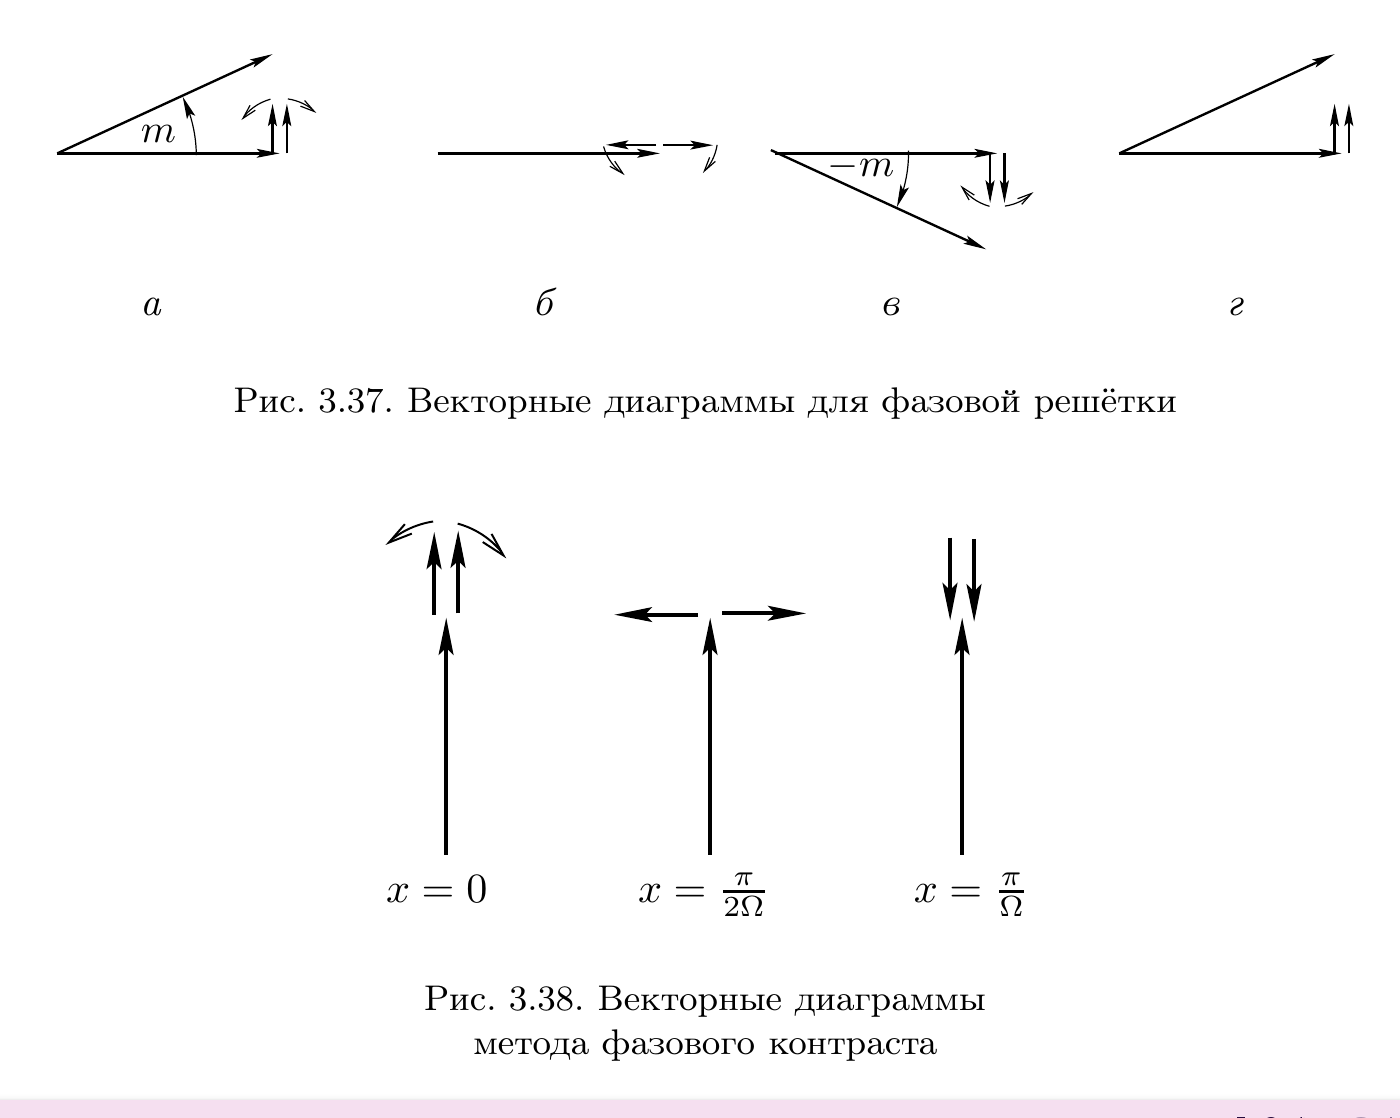
\includegraphics[width=0.8\linewidth]{../img/fk.png}}
\end{figure}

При смещении на расстояние, равное периоду решётки восстанавливается исходное расположение векторов.
 Легко  видеть, что суммарный вектор, не меняя своей длины, изменяет угол наклона
 $\varphi$ от $-m$ до $+m$, что и соответствует фазовой структуре волнового поля.

Осевая плоская волна, фокусируясь линзой в начало координат
фурье-плоскости, проходит через фазовую фильтрующую пластинку, а две наклонные волны, фокусируясь в точки
$\xi_{1,2} = \pm f\alpha = \pm f\frac{\Omega}{k}$, не задевают пластинку.
Далее линза преобразует сферические волны, исходящие из точек
$\xi = 0$ и $\xi_{1,2} = f\Omega/k$, в плоские волны, которые, интерферируя, образуют изображение.

Наличие маленькой фазовой пластинки в фурье-плоскости на оптической оси приводит к относительной фазовой задержке в
$\pi/2$ осевой волны (относительно боковых наклонных волн), поэтому поле в выходной плоскости можно записать в виде
\[
f(x) = e^{i\pi/2} + \frac{im}{2}e^{i\Omega x} + \frac{im}{2}e^{-i\Omega x}
\]
\[
f(x) = i\left(1 + m\cos\Omega x\right)
\]
Как видно из векторных диаграмм, направление суммарного вектора остаётся неизменным, а его длина при смещении по координате
$x$ изменяется, что и соответствует чисто амплитудной структуре, т. е.
полю с плоским волновым фронтом и меняющейся от точки к точке
амплитудой. Таким образом, метод фазового контраста позволяет преобразовать исходную фазовую решётку в амплитудную решётку в плоскости изображения.

Наблюдаемая картина интенсивности имеет вид
\[
I = 1 + 2m\cos\Omega x
\]

В методе тёмного поля вместо фазовой пластинки в $\pi / 2$ в фурье-плоскости на оптической оси устанавливается непрозрачный маленький экран. Осевая плоская волна, фокусируясь линзой в начало
координат фурье-плоскости, поглощается непрозрачным экраном и не
участвует в формировании изображения. Боковые же волны остаются
без изменения. Поле в выходной плоскости в этом случае имеет вид
\[
f(x) = \frac{im}{2}e^{i\Omega x} + \frac{im}{2}e^{-i\Omega x} = im\cos\Omega x
\]
А картина интенсивности
\[
I = m^2 \cos^2 \Omega x
\]

Метод тёмного поля аналогичен методу, который в радиотехнике
используется для преобразования фазовой модуляции в амплитудную
и называется приёмом без несущей.
